% !Mode:: "TeX:UTF-8"
% !TEX program  = xelatex
\documentclass[a4paper]{article}
\usepackage{amsmath}
\usepackage{amssymb}
\usepackage{ctex}
%\usepackage{braket}
%\usepackage[european]{circuitikz}
\usepackage{multirow}
\usepackage{float}
\usepackage{graphicx}
\usepackage{geometry}
\geometry{left=2.5cm,right=2.5cm,bottom=2.5cm,top=2.5cm}

\providecommand{\keywords}[1]{\textbf{关键词: #1}}

\title{近代物理实验报告10.6:居里温度测量}
\author{xy\quad 学号\quad 匡亚明学院}
\date{2019年2月29日}
\begin{document}
\maketitle
\bibliographystyle{unsrt}
%--------main-body------------

\begin{abstract}
    磁性材料在一定温度下会发生相变。温度逐渐升高时,磁性材料微观结构的有序性逐渐降低,直到某一温度材料表现为顺磁性,这个温度就称为该材料的居里温度(Curie Temperature)。本实验通过缓慢升温下测量材料的饱和磁化强度,得到$M_s - T$曲线,来确定测量的居里温度$T_c$。

    \keywords{居里温度,磁化强度}
\end{abstract}

\section{实验目的}
\begin{enumerate}
    \item 了解磁性材料居里温度的物理意义。
    \item 测定钙钛矿锰氧化物样品的居里温度。
\end{enumerate}

\section{引言}
磁性材料的自发磁化来自磁性电子间的交换作用。在磁性材料内部,交换作用总是力图使原子磁矩呈有序排列:平行取向或反平行取向。但是随着温度升高,原子热运动能量增大,逐步破坏磁性材料内部的原子磁矩的有序排列,当升高到一定温度时,热运动能和交换作用能量相等,原子磁矩的有序排列不复存在,强磁性消失,材料呈现顺磁性,此即居里温度。

不同材料的居里温度是不同的。材料居里温度的高低反映了材料内部磁性原子之间的直接交换作用、超交换作用、双交换作用。因此,深入研究和测定材料的居里温度有着重要意义。

\subsection{居里温度的测量方法}
\begin{enumerate}
    \item 通过测定材料的饱和磁化强度和温度依赖性得到$M_s$—T曲线,从而得到$M_s$降为零时所对应的居里温度。这种方法适用于那些可以用来在变温条件下直接测量样品饱和磁化强度的装置,例如磁天平、振动样品磁强计以及SQUID等。图(\ref{fig1})示出了纯Ni的饱和磁化强度的温度依赖性。由图可以确定Ni的居里温度。
          \begin{figure}[!h]
              \centering
              \begin{minipage}[!h]{0.48\textwidth}
                  \begin{center}
                      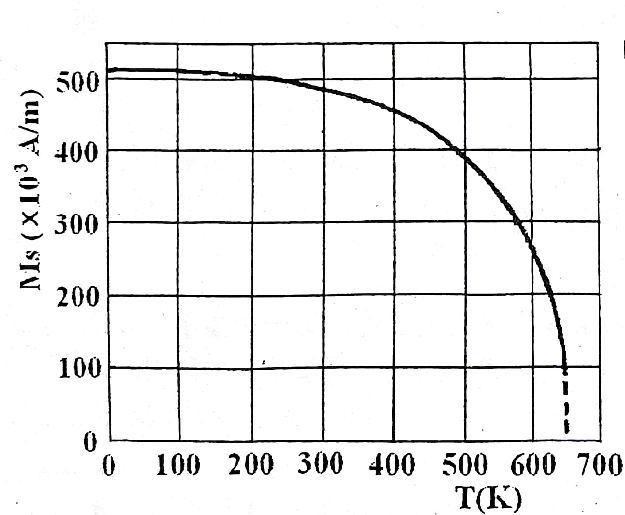
\includegraphics[width=1\textwidth]{fig/fig1.pdf}
                      \caption{纯镍的$M_s - T$曲线}\label{fig1}
                  \end{center}
              \end{minipage}
              \begin{minipage}[!h]{0.48\textwidth}
                  \begin{center}
                      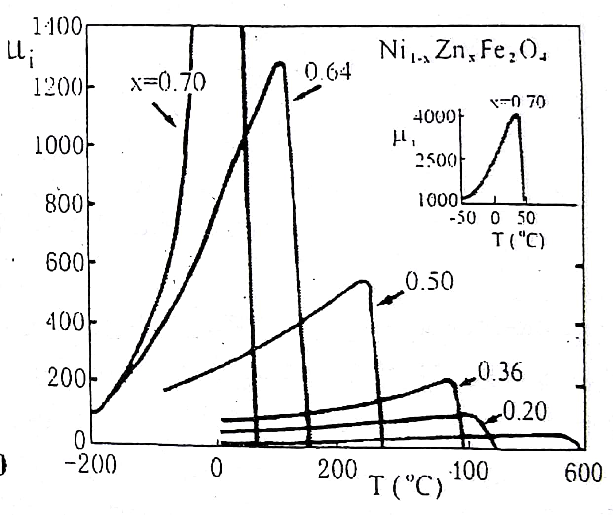
\includegraphics[width=1\textwidth]{fig/fig2.pdf}
                      \caption{镍锌铁氧体的$\mu_i - T$曲线}\label{fig2}
                  \end{center}
              \end{minipage}
          \end{figure}
    \item 通过测定材料在弱磁场下的初始磁导率$\mu_i$的温度依赖性,利用霍普金森效应,确定居里温度。霍普金森效应指的是一些软磁材料的初始磁导率在居里点附近,由于磁晶各向异性常数K1随温度升高而趋于零的速度远快于饱和磁化强度随温度的变化,而初始磁导率$\mu_i\propto\frac{M_{s2}}{K_1}$,因此在局里温度附近,$\mu_i$会显示一最大值,随后快速趋于零的现象。图(\ref{fig2})示出了不同成分的镍锌铁氧体的初始磁导率随温度的变化,这些材料的霍普金森效应十分明显。由图也可以确定各样品的居里温度。
    \item 通过测量其他磁学量(如磁致伸缩系数等)的温度依赖性求得居里温度。
    \item 通过测定一些非磁学量如比热、电阻温度系数、热电势等随温度的变化,随后根据这些非磁学量在居里温度附近的反常转折点来确定居里温度。
\end{enumerate}
\subsection{钙钛矿锰氧化物}
钙钛矿锰氧化物指的是成分为$R_{1-x}A_xMnO_3$(R是二价稀土金属离子,A为一价碱土金属离子)的一大类具有ABO$_3$型钙钛矿结构的锰氧化物。理想的ABO$_3$型(A为稀土或碱土金属离子,B为Mn离子。钙钛矿具有空间群为立方结构,如以稀土离子A作为立方晶格的顶点,则Mn离子和B离子分别处在体心和面心的位置,同时,Mn离子又位于六个氧离子组成的MnO$_6$八面体的重心,如图(\ref{fig3}-a)所示。图(\ref{fig3}-b)则是以Mn离子为立方晶格顶点的结构图。一般,把稀土离子和碱土金属离子占据的晶位称为A位,而Mn离子占据的晶位称为B位。
\begin{figure}[!h]
    \centering
    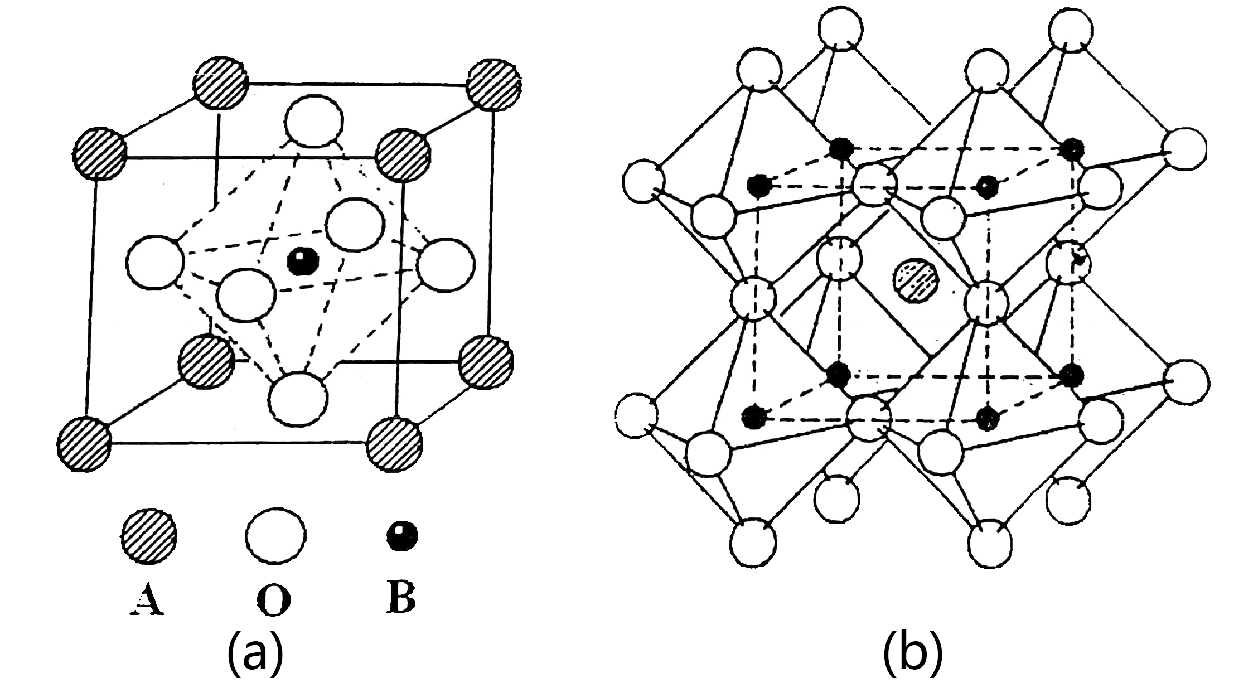
\includegraphics[width=\textwidth]{fig/fig3.pdf}
    \caption{理想的$\text{ABO}_3$钙钛矿结构}\label{fig3}
\end{figure}
这些钙钛矿锰氧化物的母本氧化物是LaMnO3,Mn离子为正二价,这是一种显示反铁磁性的绝缘体,呈理想的钙钛矿结构。早在20世纪50-60年代,人们已经发现,如果用二价碱土金属离子(Sr、Ca、Pb等)部分取代三价稀土离子,Mn离子将处于混合价状态,于是,通过和离子之间的双交换作用,在一定温度($T_p$)以下、将同时出现绝缘体—金属转变和顺磁性—铁磁性转变。随着含Sr量的增加,锰氧化物的R—T曲线形状发生明显变化。

\section{实验仪器}
信号源、锁定放大器、数字电压表、石英管、热电偶。

\section{实验原理}
\begin{figure}[!h]
    \centering
    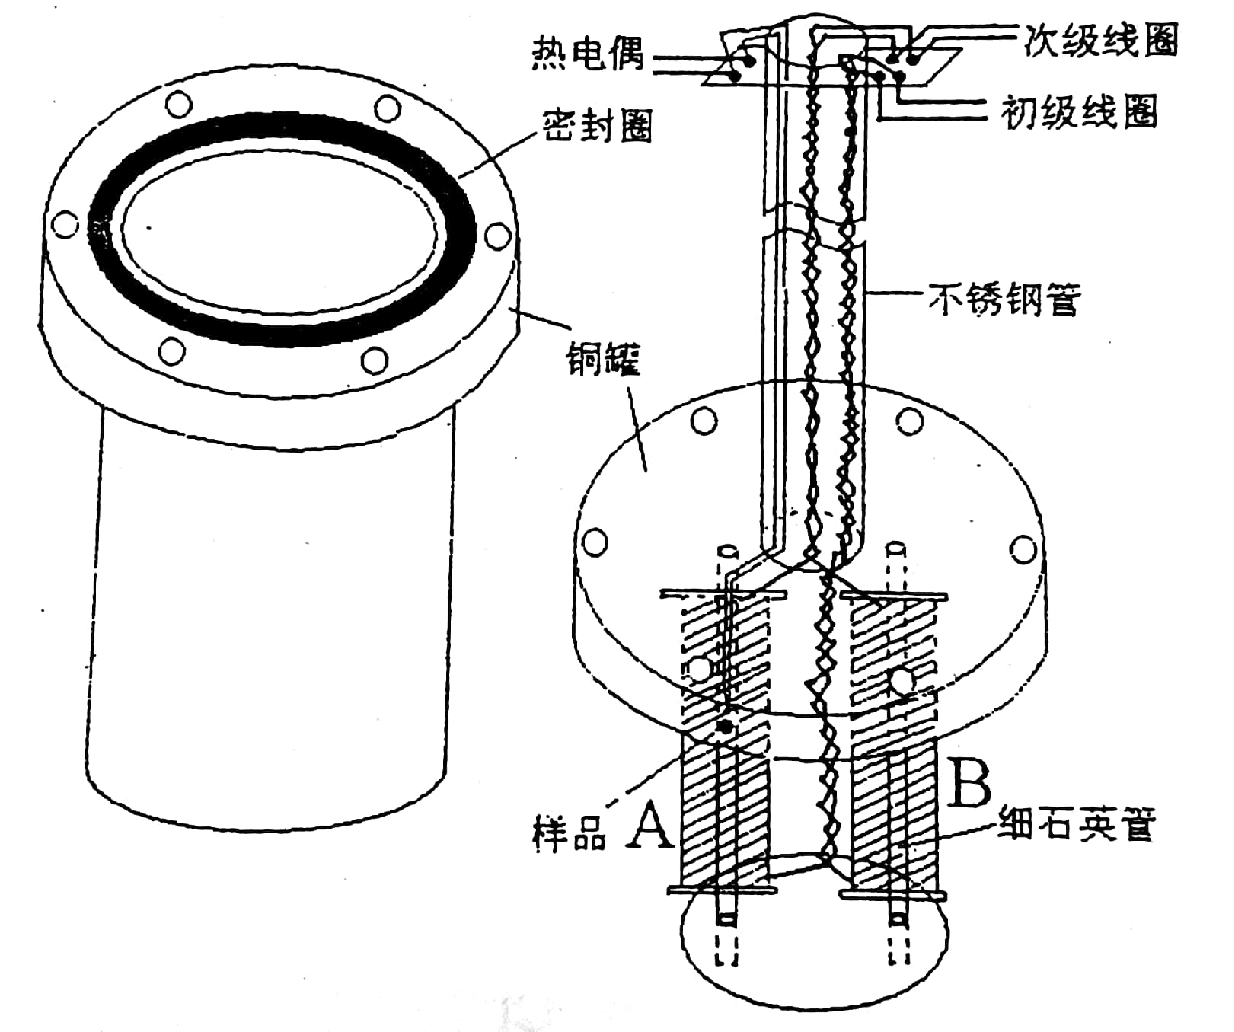
\includegraphics[width=0.75\textwidth]{fig/fig4.pdf}
    \caption{样品和测试线圈支架示意图}\label{fig4}
\end{figure}

如图(\ref{fig4})给出出了样品和测试线圈支架示意图。测试线圈由匝数和形状相同的探测线圈组A和补偿线圈组B组成。样品和热电偶置于其中一个石英管A中,另一个线圈组是作为补线圈引入的,以消除变温过程中因线圈阻抗发生的变化而造成测试误差。由于两个线圈组的次级是反串联相接的,因此其感生电动势是相互抵消的。在温度低于$T_c$时,位于探测线圈A中的钙钛矿样品呈铁磁性,而补偿线圈B中无样品,反串联的次级线圈感应输出信号强度正比于铁磁样品的磁化强度;当温度升到$T_c$以上时,探测线圈A中的钙钛矿样品呈顺磁性,和补偿线圈中空气的磁性相差无几,反串联的次级线圈感应输出信号强度几乎变为零。因此,在样品温度升高时,在$T_c$附近随着磁性的突然变化锁定放大器的输出信号强度应有一个比较陡峭的下降过程,由此可以测定居里温度$T_c$。

实验测量方框如下图所示,测试仪由信号源,锁定放大器,和数字电压表组成,测试信号频率为1.5kHz,在石英管产生的磁场约为160$\sim$400A/m,热电偶采用铜-康铜热电偶。
\begin{figure}[!h]
    \centering
    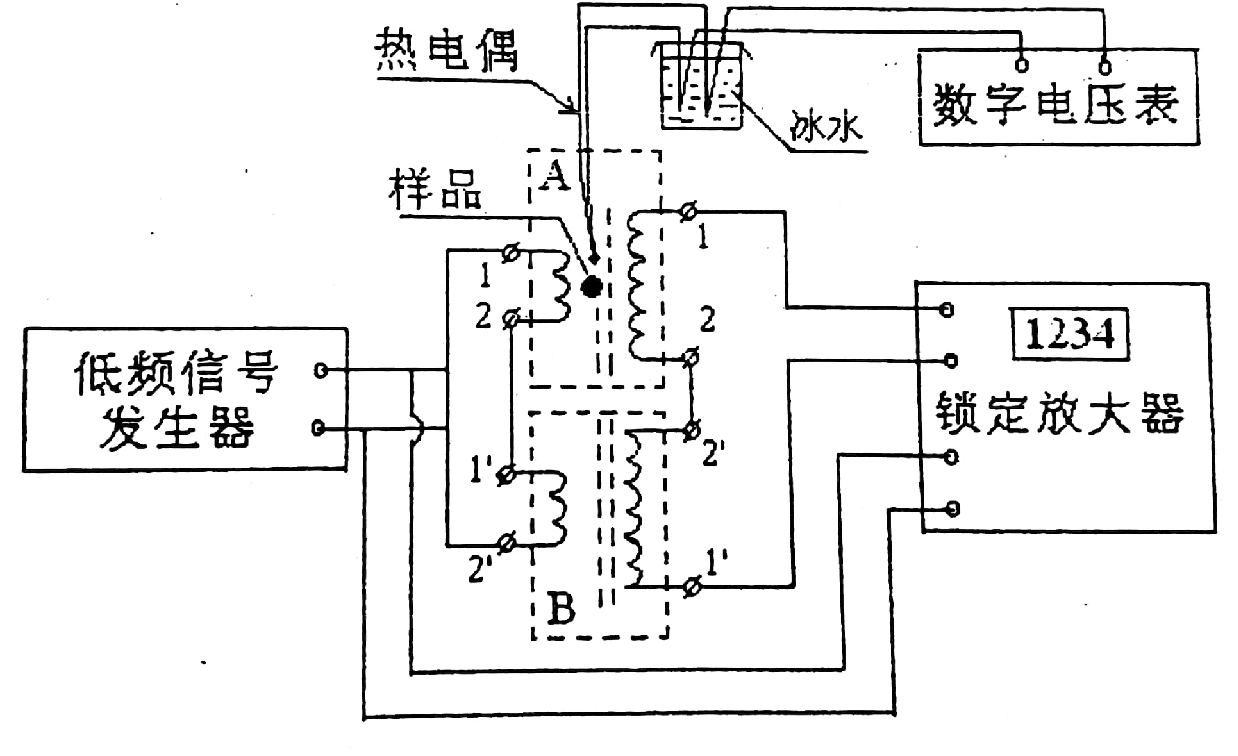
\includegraphics[width=0.8\textwidth]{fig/fig5.pdf}
    \caption{居里温度测量方框图}\label{fig5}
\end{figure}

本实验通过测定弱交变磁场下磁化强度随温度的变化来测定样品的居里温度。由于所测样品的居里温度位于77K到300K之间,因此我们设计了特有的样品和测量线圈支架。测量居里温度前,将包含这一支架的铜罐放入水中,依靠对水的加热,铜罐和样品温度逐渐升高,同时测量并记录相应于磁化强度的输出信号电压和热电偶的热电势值。以磁化强度为纵坐标、温度为横坐标作图。按照惯例,锰氧化物的居里温度被定义为$M_s - T$曲线上斜率最大点所对应的温度。

通过测定1、1$^{'}$两点间电动势的平均值,即可求出样品的磁化强度,理由如下:

对于线圈A有
\begin{equation*}
    \vec{B} = \mu_0(\vec{H}+\vec{M})
\end{equation*}
对于线圈B有
\begin{equation*}
    \vec{B} = \mu_0\vec{H}
\end{equation*}
根据法拉第电磁感应定律
\begin{equation*}
    \epsilon = -\frac{\text{d}\Phi}{\text{d}t}
\end{equation*}
分别对线圈A和线圈B有
\begin{equation*}
    \epsilon_A = -\mu_0A\left(\frac{\text{d}H}{\text{d}t} + \frac{\text{d}M}{\text{d}t}\right)
\end{equation*}
其中A是次级螺线管的横截面积,于是可得在1与1$^{'}$两端的电势差。在测量时会对1与1$^{'}$两端的电压求平均,即
\begin{equation*}
    \bar{U} = \frac{1}{T}\int_{T}U\text{d}t = -\frac{\mu_0AM}{T}
\end{equation*}
因此对1与1$^{'}$两端电压平均值的测量值,即可反映所测样品中磁化强度M的值。

\section{实验内容}
\begin{enumerate}
    \item 开启各测试仪器开关
    \item 调节低频信号器的“频率选择”为“$\times$1k”档,用“衰减调节”旋钮调节幅度,调节频率到1.5kHZ左右稳定。
    \item 设置锁定放大器的参数:放大倍数P=10,A=6,模式为“模值”。
    \item 开启搅拌器,同时开始对样品加热,不断调节水槽的加热温度,保持水与样品室温差为5摄氏度左右。搅拌器的速率不能太低也不能太高。
    \item 以0.5度为计量间隔,开始逐点测量温度和所对应的信号电压。
    \item 以归一化电压强度为纵坐标,温度为横坐标作图,并求曲线导数,最终求得居里温度。
\end{enumerate}

\section{实验数据}
实验测得的数据记录在表(\ref{data:table})中:
\begin{table}[!h]
    \centering
    \begin{tabular}{|c|c|c|c|c|c|c|c|}
        \hline
        T / $^{\circ}$C & $M_s$ / V & T / $^{\circ}$C & $M_s$ / V & T / $^{\circ}$C & $M_s$ / V & T / $^{\circ}$C & $M_s$ / V \\ \hline
        19.5            & 1.43      & 24.0            & 1.02      & 28.5            & 0.43      & 33.0            & 0.15      \\ \hline
        20.0            & 1.38      & 24.5            & 0.95      & 29.0            & 0.38      & 33.5            & 0.13      \\ \hline
        20.5            & 1.33      & 25.0            & 0.86      & 29.5            & 0.33      & 34.0            & 0.12      \\ \hline
        21.0            & 1.31      & 25.5            & 0.82      & 30.0            & 0.28      & 34.5            & 0.11      \\ \hline
        21.5            & 1.27      & 26.0            & 0.73      & 30.5            & 0.25      & 35.0            & 0.09      \\ \hline
        22.0            & 1.25      & 26.5            & 0.65      & 31.0            & 0.22      & 35.5            & 0.08      \\ \hline
        22.5            & 1.17      & 27.0            & 0.59      & 31.5            & 0.21      & 36.0            & 0.06      \\ \hline
        23.0            & 1.13      & 27.5            & 0.53      & 32.0            & 0.20      & 36.5            & 0.06      \\ \hline
        23.5            & 1.08      & 28.0            & 0.46      & 32.5            & 0.16      & 37.0            & 0.05      \\ \hline
    \end{tabular}
    \caption{实验数据}\label{data:table}
\end{table}

将表中数据和对数据的差分绘制在坐标轴中,采用样条插值(see comment) %注:应该用移动平均法(wiki: Moving Average)(thanks to: WilliamXu)
的方式对差分数据进行拟合,寻找原始数据斜率最大、即差分极小值点对应的温度,即为该材料的居里温度,如图(\ref{data:fig})所示。
\begin{figure}[!h]
\centering
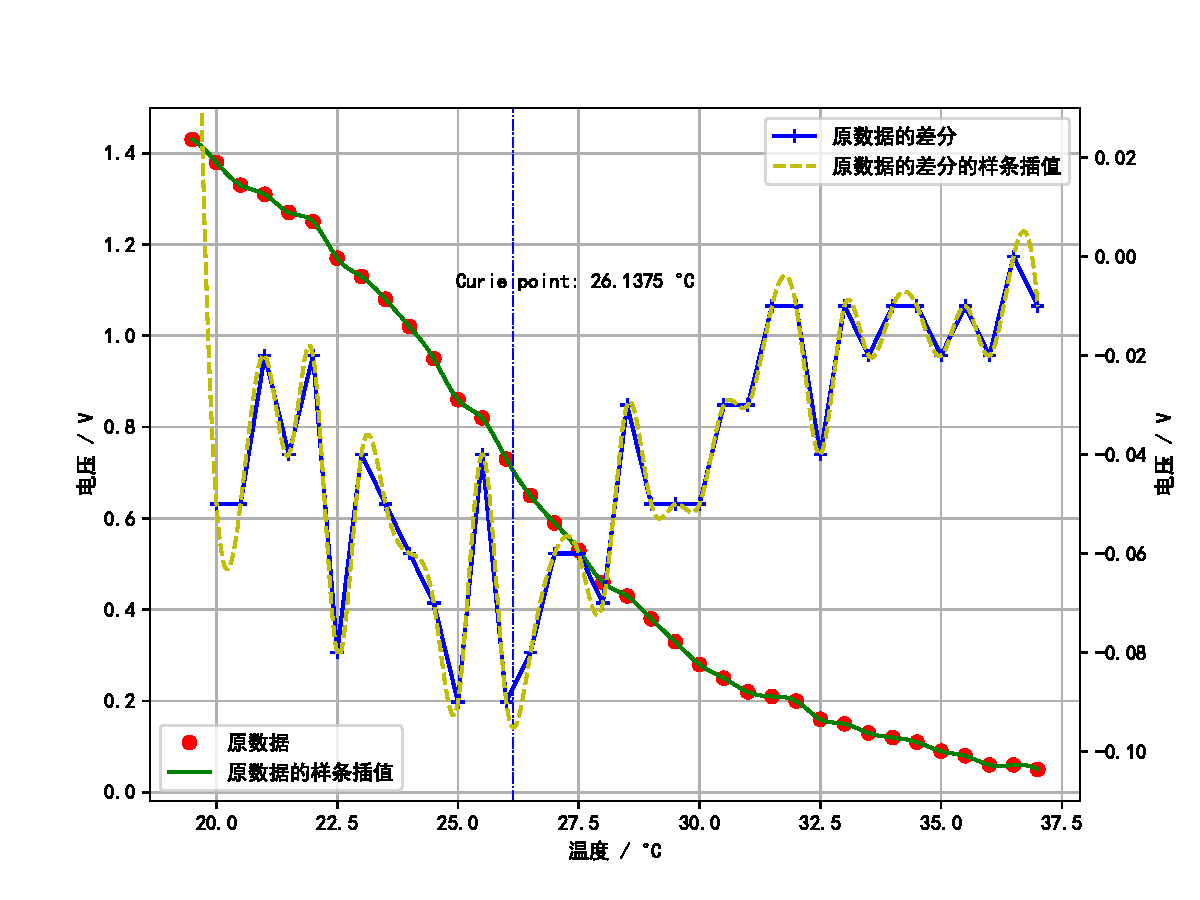
\includegraphics[width=\textwidth]{fig/data.pdf}
\caption{$M_s - T$及差分数据图像}\label{data:fig}
\end{figure}

从图(\ref{data:fig})可以得知,实验测得的该物质的居里温度$T_C\doteq 26.14 ^{\circ}$C。

\section{实验讨论}
\iffalse
对于铁磁转变为顺磁性的物质在顺磁时应满足如下的居里定律:
\begin{eqnarray*}
    \chi_m &=& \frac{C}{T-T_c}\\
    M &=& (1+\chi_m)H
\end{eqnarray*}
结合两个式子,有:
\begin{equation*}
    M = \left(1+\frac{C}{T-T_c}\right)H
\end{equation*}
化简式子,因为M与U成比例,将常数表示为A、B,得到:
\begin{equation*}
    U = A + \frac{B}{T-T_c}
\end{equation*}
用所得数据中T$>\text{T}_c$的部分作出U与$\frac{1}{T-T_c}$的函数图像,如下图:
\begin{figure}[!h]
\centering
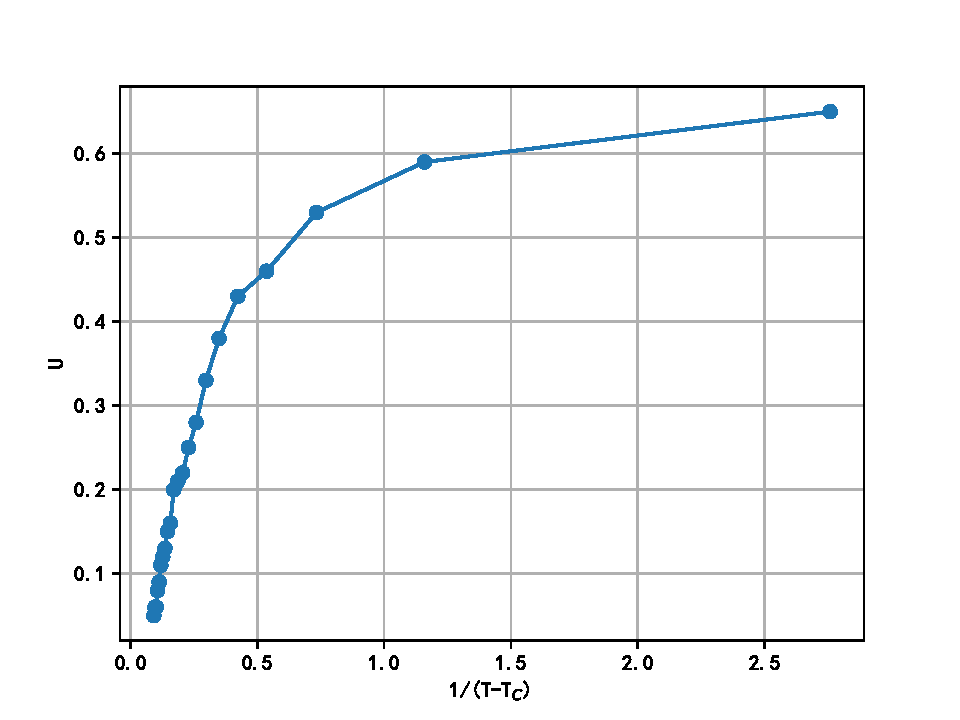
\includegraphics[width=0.8\textwidth]{fig/discussion.pdf}
\caption{$\frac{1}{T-T_C} - U$图像}\label{discussion}
\end{figure}

从图中可以看出,当U较小时,U与$\frac{1}{T-T_c}$成线性关系,H不为零。当U较大时,线性关系发生变化。猜测有两个原因,其一是U变大时,补偿线圈和探测线圈的差值逐渐变大,到时H发生变化从而改变线性关系。其二是当材料越过所标定的居里温度点时,材料并没有完全转变为顺磁材料,还保有一定的铁磁性。
\fi

\section{误差分析}
\iffalse
\begin{enumerate}
    \item 实验仪器的系统误差,由于实验仪器的精确度有所限制,所以会对实验结果产生一定的误差。
    \item 探测线圈和补偿线圈实际上并不能完全抵消。
    \item 实验中为了消除流体边界层的影响加入了搅拌来使样品均匀升温,但实验中观察到搅拌棒会引起大量气泡,实际上影响了样品表面温度。
    \item 拟合曲线时的误差。我们注意到使用不同的拟合方法得到的结果也不完全相同。
\end{enumerate}
\fi

\section{思考题}
\subsection{如果探测线圈A和补偿线圈B在绕制时不完全相同,会对测到得$M_s - T$曲线以及$T_c$产生什么影响?}

\nocite{jiaocai}
\bibliography{ref}
\end{document}